\documentclass[14pt]{article}
\usepackage[utf8]{inputenc}
\usepackage[T2A]{fontenc}
\usepackage[russian, uzbek]{babel}
\usepackage{amsmath, amssymb}
\usepackage{geometry}
\usepackage{graphicx}
\usepackage{xcolor}
\usepackage{hyperref}
\usepackage{tasks}
\usepackage{tcolorbox}
\tcbuselibrary{skins, breakable, theorems}
\usepackage{fancyhdr}
\usepackage{lastpage}
\usepackage{enumitem}
\usepackage{paracol} 
\usepackage{ifthen}
\usepackage{needspace}

% Tangens va kotangens uchun buyruqlar
\newcommand{\tg}{\operatorname{tg}}
\newcommand{\ctg}{\operatorname{ctg}}

% Geometriya sozlamalari
\geometry{a4paper, left=10mm, right=10mm, top=20mm, bottom=20mm, headheight=15pt}

% Ranglar palitrasi
\definecolor{primary}{RGB}{52, 152, 219}       % To'q ko'k
\definecolor{secondary}{RGB}{46, 204, 113}     % Yashil
\definecolor{accent}{RGB}{155, 89, 182}        % Binafsha
\definecolor{lightbg}{RGB}{248, 249, 250}      % Och kulrang fon
\definecolor{taskborder}{RGB}{230, 230, 230}   % Vazifa chegarasi rangi
\definecolor{optionbg}{RGB}{240, 242, 245}     % Variantlar foni

% Sahifa foni
\pagecolor{lightbg}

% Giperssilka sozlamalari
\hypersetup{
    colorlinks=true,
    linkcolor=primary,
    urlcolor=primary,
}

% Kolontitullar
\pagestyle{fancy}
\fancyhf{}
\fancyhead[L]{\textcolor{primary}{\textbf{MathCore | MOCK Test-5}}}
\fancyhead[R]{\textcolor{secondary}{Abdunazarov M.X.}}
\fancyfoot[L]{\href{https://t.me/Math_Core_Dtm_MS_Att}{\textcolor{primary}{MathCore}}}
\fancyfoot[R]{\href{https://t.me/Abd_mardon}{\textcolor{secondary}{@Abd\_mardon}}}
\fancyfoot[C]{\textcolor{gray}{\thepage/\pageref{LastPage}}}
\renewcommand{\headrulewidth}{0.5pt}
\renewcommand{\headrule}{\hbox to\headwidth{\color{primary}\leaders\hrule height \headrulewidth\hfill}}
\renewcommand{\footrulewidth}{0.5pt}
\renewcommand{\footrule}{\hbox to\headwidth{\color{secondary}\leaders\hrule height \footrulewidth\hfill}}

% Sarlavha sahifasi
\title{\Huge \textbf{\textcolor{primary}{MOCK Test-5}}}
\author{\textcolor{secondary}{Abdunazarov M.X.}}
\date{}

% Savol kartochkasi stili
\newtcolorbox{questionbox}[2][]{
    enhanced,
    breakable,
    colback=white,
    colframe=primary,
    coltitle=white,
    fonttitle=\bfseries\large,
    title={Masala \hfill \textcolor{white}{#2}},
    attach boxed title to top left={xshift=5mm, yshift=-2mm},
    boxed title style={size=small, colback=primary, sharp corners},
    sharp corners,
    boxrule=0.5pt,
    left=5mm,
    right=5mm,
    top=5mm,
    bottom=5mm,
    drop fuzzy shadow,
    #1
}

% Javob variantlari stili
\newlist{options}{enumerate}{1}
\setlist[options]{
    label=\textbf{\Alph*)},
    leftmargin=*,
    itemsep=2pt,
    topsep=5pt,
    before={\vspace{2mm}\begin{tcolorbox}[
        colback=optionbg,
        colframe=white,
        sharp corners,
        boxrule=0pt,
        left=2mm,
        right=2mm,
        top=2mm,
        bottom=2mm,
    ]},
    after={\end{tcolorbox}\vspace{2mm}},
}

% Rasmlar uchun
\newcommand{\questionimage}[2][0.5\linewidth]{%
    \begin{center}
        \includegraphics[width=#1]{#2}
    \end{center}
}

\begin{document}

\maketitle
\begin{center}
    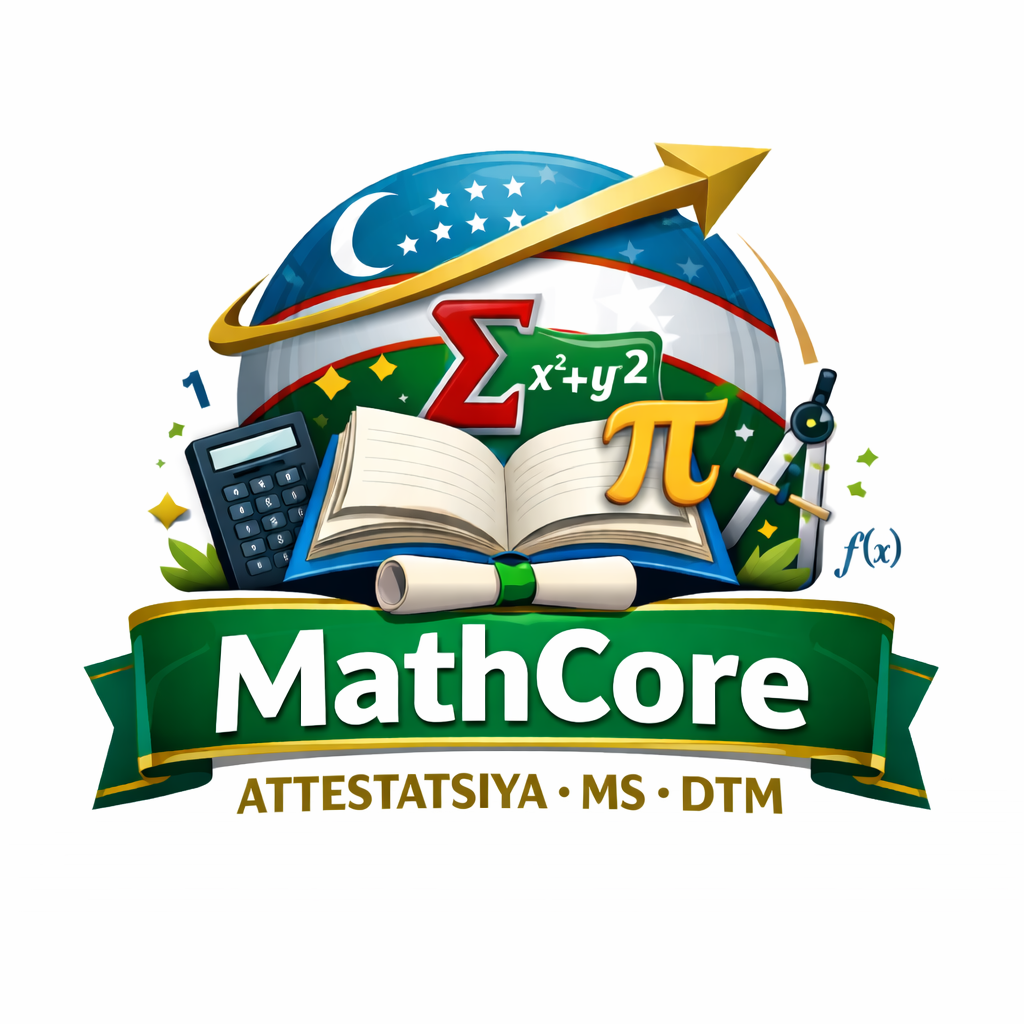
\includegraphics[width=0.2\textwidth]{logo.png} \\[5mm]
    \textcolor{gray}{\small Telegram: \href{https://t.me/Math_Core_Dtm_MS_Att}{@Math\_Core\_Dtm\_MS\_Att}}
\end{center}
\vspace{5mm}

\columnratio{0.48,0.48}
\setlength{\columnsep}{0.04\textwidth}

% Masala 1
\begin{questionbox}{1}
    Agar \( x^3 - 15^3 = 9^3 + 12^3 \) bo'lsa, \( x \) ni toping.
    \begin{options}
        \item 21
        \item 28
        \item 20
        \item 18
    \end{options}
\end{questionbox}

% Masala 2
\begin{questionbox}{2}
    Hisoblang: \[\frac{1+2}{2} + \frac{1+2+3}{2^2} + \frac{1+2+3+4}{2^3} + \cdots\]
    \begin{options}
        \item \(\frac{28}{4}\)
        \item \(\frac{7}{2}\)
        \item \(\frac{7}{4}\)
        \item \(\frac{3}{2}\)
    \end{options}
\end{questionbox}

% Masala 3
\begin{questionbox}{3}
    Agar \( x^2 + 5, \frac{1}{2} \sin \frac{\pi x}{4} \) va \(-4x\) sonlari arifmetik progressiyaning ketma-ket hadlari bo'lsa, \( x \) nechta turli qiymat qabul qilishi mumkin?
    \begin{options}
        \item 0
        \item 1
        \item 2
        \item 3
    \end{options}
\end{questionbox}

% Masala 4
\begin{questionbox}{4}
    Qisqarmaydigan \(\frac{a}{b}\) kasrning suratiga 14, maxrajiga esa 35 qo'shildi va \(\frac{c}{d}\) kasr hosil bo'ldi. Agar \( ad = bc \) bo'lsa, \( a + b \) ning qiymatini toping.
    \begin{options}
        \item 14
        \item 7
        \item 49
        \item aniqlab bo'lmaydi
    \end{options}
\end{questionbox}

% Masala 5
\begin{questionbox}{5}
    Chizmada zınapoyaning \( n \) ta pog'onasi hamda ularga joylashtirilgan qizil va yashil sharlar ko'rsatilgan. Agar sharlarning umumiy soni 210 ta bo'lsa, qizil sharlar soni nechta?
    \questionimage{1.png}
    \begin{options}
        \item 105
        \item 110
        \item 112
        \item 115
    \end{options}
\end{questionbox}

% Masala 6
\begin{questionbox}{6}
    Agar \( n^n \) soni 3001 ta raqamdan iborat bo'lsa, \( n \) natural sonida nechta raqam bor?
    \begin{options}
        \item 2
        \item 3
        \item 4
        \item 5
    \end{options}
\end{questionbox}

% Masala 7
\begin{questionbox}{7}
    Birinchi qotishma tarkibida 65\% oltin va 35\% kumush bor. Ikkinchi qotishma tarkibida 40\% oltin va 60\% kumush bor. Tarkibida 50\% oltin bo'lgan 8 kg qotishma olish uchun birinchi qotishmadan necha kg olish kerak?
    \begin{options}
        \item 3,1(9)
        \item \(3\frac{2}{5}\)
        \item 4,8
        \item \(3\frac{2}{15}\)
    \end{options}
\end{questionbox}

% Masala 8
\begin{questionbox}{8}
    \( f(x) = ax^2 + bx + c \) funksiya \( Ox \) o'qiga urinadi. Agar simmetriya o'qi tenglamasi \( x = 3 \) bo'lsa, \( \frac{c}{a} \) ning qiymatini toping.
    \begin{options}
        \item \(\frac{1}{9}\)
        \item 9
        \item \(-\frac{1}{9}\)
        \item aniqlab bo'lmaydi
    \end{options}
\end{questionbox}

% Masala 9
\begin{questionbox}{9}
    \(-71\) sonini 6 ga bo'lgandagi qoldiqni toping.
    \begin{options}
        \item \(-5\)
        \item 1
        \item 5
        \item \(-1\)
    \end{options}
\end{questionbox}

% Masala 10
\begin{questionbox}{10}
    Chizmada \( y = x^2 + nx + k \) funksiyaning grafigi tasvirlangan bo'lib, uning eng kichik qiymati \(-1\) ga teng. Chizmadagi ma'lumotlardan foydalanib, \( n + k \) ni toping.
    \questionimage{2.png}
    \begin{options}
        \item 7
        \item 4
        \item 5
        \item 6
    \end{options}
\end{questionbox}

% Masala 11
\begin{questionbox}{11}
    Imtihonda 36 ta savol bor: 21 ta qiyin va 15 ta oson. Agar birinchi bo'lib kirgan talabaga qiyin savol tushgani ma'lum bo'lsa, to'rtinchi bo'lib kirgan talabaga oson savol tushishi ehtimolligini toping.
    \begin{options}
        \item \(\frac{5}{12}\)
        \item \(\frac{1}{2}\)
        \item \(\frac{3}{7}\)
        \item 0,6
    \end{options}
\end{questionbox}

% Masala 12
\begin{questionbox}{12}
    Agar $(x - 1)^3(2x - 1)^7 = a + a_1x + a_2x^2 + \cdots + a_{10}x^{10}$ bo'lsa, $a + a_1$ ni toping.
    \begin{options}
        \item $-10$
        \item $-16$
        \item $-14$
        \item $-17$
    \end{options}
\end{questionbox}

% Masala 13
\begin{questionbox}{13}
    Agar \( x_1, x_2 \) va \( x_3 \) sonlari \( x^3 + 3x - 1 = 0 \) tenglamasining ildizlari bo'lsa, \( x_1x_2(x_1 + x_2) + x_1x_3(x_1 + x_3) + x_2x_3(x_2 + x_3) \) ifodaning qiymatini toping.
    \begin{options}
        \item 0
        \item $-3$
        \item 1
        \item $-1$
    \end{options}
\end{questionbox}

% Masala 14
\begin{questionbox}{14}
    Agar \( k = 2^{2022} \) bo'lsa, \( 7^{8k+3} \) sonini 15 ga bo'lgandagi qoldiqni toping.
    \begin{options}
        \item 12
        \item 13
        \item 4
        \item 11
    \end{options}
\end{questionbox}

% Masala 15
\begin{questionbox}{15}
    Agar \( a = \frac{\sqrt{3}(3+2\sqrt{3})}{4} \) bo'lsa, \( \frac{2}{1-\frac{2}{2+\frac{1}{a-2}}} \) ifodaning qiymatini toping.
    \begin{options}
        \item \(3\sqrt{3}\)
        \item \(\frac{3\sqrt{3}+1}{2}\)
        \item \(3\sqrt{3} + 2\)
        \item \(\sqrt{3}\)
    \end{options}
\end{questionbox}

% Masala 16
\begin{questionbox}{16}
    Agar \( ABCDA_1B_1C_1D_1 \) kub bo'lsa, \( A_1A - C_1D + BC \) vektoriga teng bo'lgan vektorni aniqlang.
    \begin{options}
        \item \(BD\)
        \item \(B_1C\)
        \item \(B_1A_1\)
        \item \(AC\)
    \end{options}
\end{questionbox}

% Masala 17
\begin{questionbox}{17}
    Chizmada \( y = x^2 + 2 \) va \( y = \frac{3}{x} \) funksiyalarining grafiklari tasvirlangan. Chizmadagi ma'lumotlardan foydalanib, bo'yalgan soha yuzini toping.
    \questionimage{3.png}
    \begin{options}
        \item \(\frac{1}{4}\)
        \item \(\frac{2}{3}\)
        \item \(\frac{4}{5}\)
        \item \(\frac{4}{3}\)
    \end{options}
\end{questionbox}

% Masala 18
\begin{questionbox}{18}
    Arifmetik progressiyada \( a_{30} = 3 \) va \( a_{32} = 11 \). Progressiya dastlabki \( n \) ta hadining yig'indisi qabul qilishi mumkin bo'lgan eng kichik qiymatni toping.
    \begin{options}
        \item \(-1647\)
        \item \(-1652\)
        \item \(-1653\)
        \item \(-1650\)
    \end{options}
\end{questionbox}

% Masala 19
\begin{questionbox}{19}
    Sardor Salohiddinovning matematika bo'yicha testlar to'plami sahifalarini 3-betdan boshlab raqamlash uchun jami 3523 ta raqam ishlatildi. To'plamda nechta sahifa bor?
    \begin{options}
        \item 1158
        \item 1112
        \item 1113
        \item 1159
    \end{options}
\end{questionbox}

% Masala 20
\begin{questionbox}{20}
    Uchta idishda jami 18 litr suv bor. Birinchi idishdagi suvning yarmini ikkinchisiga, so'ng ikkinchi idishda hosil bo'lgan suvning uchdan bir qismini uchinchisiga va nihoyat uchinchi idishdagi suvning to'rtdan bir qismini birinchisiga quyishdi. Shundan so'ng barcha idishlarda suv miqdori teng bo'lib qoldi. Dastlab har bir idishda necha litrdan suv bo'lgan?
    \begin{options}
        \item 8; 5; 5
        \item 3; 7; 8
        \item 6; 6; 6
        \item 4; 8; 6
    \end{options}
\end{questionbox}

% Masala 21
\begin{questionbox}{21}
    Agar \(\cos(4x - 10^\circ) = -\frac{\sqrt{3}}{2}\) bo'lsa, \( x \) ning eng kichik natural qiymatini (gradusda) toping.
    \begin{options}
        \item 25
        \item 30
        \item 40
        \item 45
    \end{options}
\end{questionbox}

% Masala 22
\begin{questionbox}{22}
    Aylanadagi 5 ta nuqtani tutashtirib nechta turli vatar o'tkazish mumkin?
    \begin{center}
        
\includegraphics[width=0.2\textwidth]{4.png}
    \end{center}
    \begin{options}
        \item 5
        \item 4
        \item 10
        \item 8
    \end{options}
\end{questionbox}

% Masala 23
\begin{questionbox}{23}
    Umumiy hadi  \( 
    a_n = \frac{(n-1)!}{n^2 - n} \)  bo'lgan ketma-ketlik berilgan, bo'lsa   \( \frac{a_{n+1}}{a_n} \) nimaga teng.
    \begin{options}
        \item \(\frac{n(n-1)}{n+1}\)
        \item \(\frac{n+1}{2n}\)
        \item \(\frac{n(n+2)}{2n+2}\)
        \item \(\frac{2n}{n-1}\)
    \end{options}
\end{questionbox}

% Masala 24
\begin{questionbox}{24}
    Qutida 4 ta qora va 5 ta oq shar bor. Tasodifiy tanlangan ikkita sharning ikkalasi ham oq bo'lish ehtimolligini toping.
    \begin{options}
        \item \(\frac{5}{18}\)
        \item \(\frac{2}{9}\)
        \item \(\frac{1}{6}\)
        \item \(\frac{1}{3}\)
    \end{options}
\end{questionbox}

% Masala 25
\begin{questionbox}{25}
    Qaysi variantda ko'rsatkichli funksiya keltirilgan?
    \begin{options}
        \item \((3\sqrt{-2})^x\)
        \item \((-2)^x\)
        \item \(3^{-x}\)
        \item \(1^x\)
    \end{options}
\end{questionbox}

% Masala 26
\begin{questionbox}{26}
    \( 4^{\sqrt{2x+5}} - 10 \cdot 2^{\sqrt{2x+5}} + 16 > 0 \) tengsizlikning eng kichik natural yechimini toping.
    \begin{options}
        \item 2
        \item 3
        \item 1
        \item 4
    \end{options}
\end{questionbox}

% Masala 27
\begin{questionbox}{27}
    Chizmada to'g'ri burchakli \( ABC \) uchburchak tasvirlangan. Agar \( AB = \log_{27} 16 \) va \( AC = \log_2 81 \) bo'lsa, \( ABC \) uchburchak yuzini toping.
    \questionimage{5.png}
    \begin{options}
        \item \(\frac{16}{3}\)
        \item 4
        \item \(\frac{8}{3}\)
        \item 2
    \end{options}
\end{questionbox}

% Masala 28
\begin{questionbox}{28}
    ABCD kvadratining yuzi 36 ga teng bo'lib, AB tomoni abssissa o'qiga parallel. Agar A, B va C uchlari mos ravishda \( y = \log_a x \), \( y = 2 \log_a x \) va \( y = 3 \log_a x \) funksiyalarining grafiklarida yotsa, \( a \) ning qiymatini toping.
    \begin{options}
        \item \(\sqrt[6]{3}\)
        \item \(\sqrt[3]{3}\)
        \item \(\sqrt[3]{6}\)
        \item \(\sqrt[6]{6}\)
    \end{options}
\end{questionbox}

% Masala 29
\begin{questionbox}{29}
    Tomoni 1 ga teng bo'lgan ikkita kvadrat ustma-ust qo'yilgan. So'ngra kvadratlardan biri ularning umumiy simmetriya markazi atrofida 45° ga burildi. Hosil bo'lgan shaklning yuzini toping.
    \begin{options}
        \item \(4 - 2\sqrt{2}\)
        \item \(4 - \sqrt{2}\)
        \item 1,2
        \item 2,5
    \end{options}
\end{questionbox}

% Masala 30
\begin{questionbox}{30}
    Chizmada \( y = 9 - x^2 \) funksiyaning grafigi tasvirlangan. Chizmadagi ma'lumotlardan foydalanib, ABCD to'rtburchak yuzining eng katta qiymatini toping.
    \questionimage{6.png}
    \begin{options}
        \item \(12\sqrt{3}\)
        \item \(9\sqrt{3}\)
        \item \(6\sqrt{3}\)
        \item 12
    \end{options}
\end{questionbox}

% Masala 31
\begin{questionbox}{31}
    $OP = 8$ sm, $PA = 2$ sm, $OB = 10$ sm. Asosining markazi $O$ va radiusi 10 sm bo'lgan to'g'ri konusning asosiga parallel tekislik uni kesib o'tib, asosining markazi $P$ va radiusi 2 sm bo'lgan kesik konus hosil qiladi. Chizmadagi kesik konusning yon sirti yuzini toping.
    \questionimage{36.png}
    \begin{options}
        \item $36\sqrt{2}$
        \item $72\sqrt{2}$
        \item $84\sqrt{2}$
        \item $96\sqrt{2}$
    \end{options}
\end{questionbox}

% Masala 32
\begin{questionbox}{32}
    Asosining radiusi 8 dm va balandligi 25 dm bo'lgan silindrsimon idishga ma'lum miqdorda suv quyilgan. Agar $OH = 4\sqrt{2}$ dm bo'lsa, idishda necha litr suv bor? ($\pi = 3$ deb oling)
    \questionimage{37.png}
    \begin{options}
        \item 400
        \item 480
        \item 500
        \item 520
    \end{options}
\end{questionbox}

% Masala 33
\begin{questionbox}{33}
    $O$ nuqta kvadrat asosli to'g'ri piramidaning og'irlik markazi. $TE = \sqrt{5}$ sm, $AE = 2\sqrt{5}$ sm, $AB = 6$ sm. Piramidaning $O$ nuqtasida turgan chumoli piramida sirti bo'ylab $E$ nuqtaga eng qisqa yo'l bilan borishi mumkin. Bu masofa qancha?
    \questionimage{38.png}
    \begin{options}
        \item $\sqrt{38}$
        \item $3\sqrt{5}$
        \item 7
        \item $5\sqrt{2}$
    \end{options}
\end{questionbox}

% Masala 34
\begin{questionbox}{34}
    $TK = 7$ sm, $AK = 17$ sm, $OB = 6$ sm. Ushbu to'g'ri konusning $A$ nuqtasida turgan chumoli konus sirti bo'ylab $K$ nuqtaga eng qisqa yo'l bilan borishi uchun necha sm yo'l yurishi kerak?
    \questionimage{39.png}
    \begin{options}
        \item 25
        \item 26
        \item 27
        \item 28
    \end{options}
\end{questionbox}

% Masala 35
\begin{questionbox}{35}
    $A = \{(x,y): x \geq 0, x + y \geq 1, 4x + y \leq 4\}$ to'plamni $y$ o'qi atrofida 360° ga aylantirishdan hosil bo'lgan jismning hajmini toping:
    \begin{options}
        \item $\pi$
        \item $\frac{4}{3}\pi$
        \item $\frac{3}{2}\pi$
        \item $\frac{5}{3}\pi$
    \end{options}
\end{questionbox}

\end{document}